% !TEX root = ../intro-stellar-physics.tex

Hot air rises, as a glider pilot or hawk can tell you. The fluid velocities in question are very subsonic, so we have hydrostatic equilibrium to excellent approximation. But the fluid motions make an enormous difference for heat transport! This state of fluid motions induced by a temperature gradient is known as \newterm{convection}. You can perform the following demonstration of the onset of convection.  Brew tea, and pour the hot tea into a saucepan that is on an unlit burner.  Use a straw with your thumb over the top to insert a layer of cold milk under the warm tea in the saucepan.  The temperature difference between the tea and milk will inhibit their mixing. Light the burner, and watch for the development of convection---you will know it when you see it.

\begin{figure}[htbp]
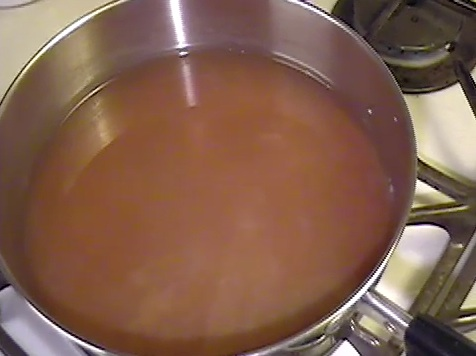
\includegraphics[width=0.5\linewidth]{convection-1}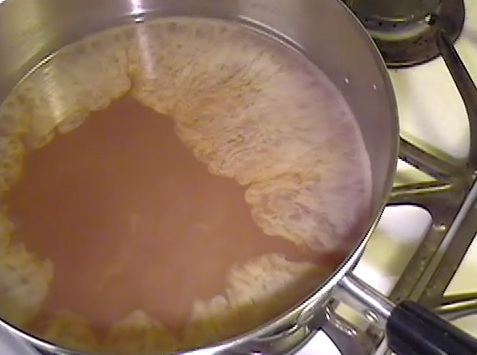
\includegraphics[width=0.5\linewidth]{convection-2}
\caption{Onset of convection in a tea-milk mixture.\label{f.tea}}
\end{figure}

\section{The adiabatic thermal gradient}\label{s.adiabatic-gradient}

We saw that the temperature gradient in the star is (eq.~[\ref{e.gradient-temperature}])
\[
    \DD{T}{r} = -\frac{3\rho\kappa}{4acT^3}\frac{L(r)}{4\pi r^2}.
\]
Here $\kappa$ is the opacity and $L(r)$ is the luminosity at radius $r$: $L/4\pi r^2$ is the flux. If this thermal gradient, $|\dif T/\dif r|$, becomes too large, however, the fluid becomes unstable: warm fluid begins to rise while cold fluid sinks to take its places.  This usually occurs quickly enough that there is little exchange of heat between the upwelling warm current and the sinking cold one.

As a result of this lack of heat exchange, the motions are termed \newterm{adiabatic}.  To understand what this means, recall the first law of thermodynamics\cite{Fermi1956Thermodynamics}, which relates the change in internal energy $\dif U$ and in volume $\dif V$ to the heat transferred $\dif Q$:
\begin{equation}\label{e.first-law-thermo}
	\dif Q = \dif U + P\dif V,
\end{equation}
where $P$ is the pressure. Now, we aren't using volume to describe our fluid so let's apply this equation to a fixed mass of fluid, say $m = \val{1}{\kilo\gram}$, and divide both sides of Equation~(\ref{e.first-law-thermo-astro}) by the mass. Then $Q$ refers to the heat transferred \emph{per kilogram}, and $U$ refers to the internal energy \emph{per kilogram}.  Instead of $\dif V$, we then have $\dif(V/m) = \dif(1/\rho) = -\rho^{-2}\dif\rho$.  Our first law, rewritten in terms of mass-specific quantities, is thus
\begin{equation}\label{e.first-law-thermo-astro}
	\dif Q = \dif U -\frac{P}{\rho^{2}}\dif \rho.
\end{equation}
Suppose we wish to express quantities in terms of temperature $T$ and density $\rho$: then
\[ \dif U = \tderiv{U}{T}{\rho}\dif T + \tderiv{U}{\rho}{T}\dif \rho, \]
and
\[ \dif Q = \tderiv{U}{T}{\rho}\dif T + \left[\tderiv{U}{\rho}{T} - \frac{P}{\rho^{2}}\right]\dif \rho. \]
Hence the heat needed to raise the temperature of one kilogram of fluid when holding density fixed is
\begin{equation}\label{e.CV}
C_{\rho} \equiv \tderiv{Q}{T}{\rho} = \tderiv{U}{T}{\rho}.
\end{equation}
For an ideal gas, $U = U(T)$ and $C_{\rho}$ is approximately constant; hence we may integrate equation~(\ref{e.CV}) to obtain $U = C_{\rho}T + \textrm{const}$.

In Eq.~(\ref{e.first-law-thermo-astro}), the last term is $-(P/\rho)\, (\dif\rho/\rho) = -(P/\rho)\,\dif\ln\rho$. This demonstrates a useful trick: take the logarithm of the equation of state, $\ln (P) = \ln(\rho) + \ln (T) + \ln (\kB/\mu\mb)$, and then take the differential to obtain
\[ \frac{\dif P}{P} = \frac{\dif\rho}{\rho} + \frac{\dif T}{T}. \]
Now eliminate $\dif\rho/\rho$ in the equation
\[ \dif Q = C_{\rho}\dif T - \frac{P}{\rho}\frac{\dif\rho}{\rho} \]
to obtain an expression for the heat transferred as a function of temperature and pressure,
\[ \dif Q = \left[C_{\rho} + \frac{P}{\rho T}\right]\dif T - \frac{1}{\rho}\dif P
	 = \left[C_{\rho} + \frac{\kB}{\mu\mb}\right]\dif T - \frac{1}{\rho}\dif P. \]
From this we see that the heat needed to raise the temperature of one kilogram when holding pressure fixed is
\begin{equation}\label{e.CP}
C_{P}\equiv \tderiv{Q}{T}{P} = C_{\rho} + \frac{\kB}{\mu\mb}.
\end{equation}
For a plasma of ions and electrons, $C_\rho = (3/2)\kB/(\mu\mb)$ and hence $C_P = (5/2)\kB/(\mu\mb)$.  The ratio of specific heats is
\begin{equation}\label{e.gamma}
    \gamma = \frac{C_P}{C_\rho} = \frac{5/2}{3/2} = \frac{5}{3}.
\end{equation}
This value of $\gamma$ is for an ideal gas and does not hold universally.

\newthought{During adiabatic motion, there is no heat exchange:} hence, the entropy is constant,
\begin{equation}\label{e.differential-entropy}
    T\dif S = \dif Q = 0 = C_{P}\dif T - \frac{1}{\rho} \dif P.
\end{equation}
Using the ideal gas equation of state we can write 
\[
    \frac{1}{\rho} = \frac{\kB}{\mu\mb} \frac{T}{P}
\]
and insert this into Equation~(\ref{e.differential-entropy}) to obtain
\begin{equation}\label{e.differential-adiabat}
     \frac{\dif T}{T} = \frac{\kB/(\mu\mb)}{C_{P}}\frac{\dif P}{P} = \frac{C_{P}-C_{\rho}}{C_{P}} \frac{\dif P}{P} = \frac{\gamma-1}{\gamma}\frac{\dif P}{P}.
\end{equation}
Integrating both sides of the equation gives
\[ \ln T = \frac{\gamma-1}{\gamma}\ln P + \textrm{const.},\]
or 
\begin{equation}\label{e.adiabat}
 T = T_{0}\left(\frac{P}{P_{0}}\right)^{(\gamma-1)/\gamma},
\end{equation}
where $T_{0}$ and $P_{0}$ are the temperature and pressure at the beginning of the adiabatic process.
Equation~(\ref{e.adiabat}) tells us how the temperature changes with pressure along an adiabat for an ideal gas.  Notice that we can recast Equation~(\ref{e.differential-adiabat}) as
\begin{equation}
    \frac{P}{T}\left(\dd{T}{P}\right)_s = \left(\dd{\ln T}{\ln P}\right)_s = \frac{\gamma-1}{\gamma}.
\label{e.nabla-adiabat}
\end{equation}
Equation~(\ref{e.nabla-adiabat}) tells us how temperature changes with pressure in an adiabatically stratified gas.

\section{The onset of convection}\label{s.convection-onset}

To understand when convection starts, let's consider a fluid in planar geometry and hydrostatic equilibrium,
\begin{equation}
\frac{\dif P}{\dif r} = -\rho g.
\end{equation}
Now, imagine moving a blob of fluid upwards from $r$ to $r+h$.  We move the blob slowly enough that it is in hydrostatic equilibrium with its new surroundings, $P_{b}(r+h) = P(r+h)$, where the subscript $b$ refers to ``blob.'' We do move the blob quickly enough, however,  that it does not remain in \emph{thermal} equilibrium with its surroundings; that is, we move the blob \emph{adiabatically}.  The entropy of the blob is therefore constant, 
$S_{b}(r+h) = S_{b}(r) = S(r)$, and is therefore not, in general, equal to the entropy of the surrounding gas at $r+h$: $S_{b}(r+h)  \neq S(r+h)$.  

As the blob rises, it displaces some of the surrounding fluid. Archimedes tells us that if the displaced fluid is less massive than the blob, then the blob will sink.  We can rephrase this in terms of the volume occupied by a unit mass of fluid $V$: if the volume occupied by the blob is less than the volume of an equal mass of background, then the blob will sink. Translating this into an equation: if
\begin{eqnarray}
\lefteqn{V[P(r+h),S(r+h)] - V_{b}[P_{b}(r+h),S_{b}(r+h)] =}\nonumber\\
&&  V[P(r+h),S(r+h)] - V[P(r+h),S(r)] > 0
\label{e.archimedes}
\end{eqnarray}
then the blob will sink. If condition (\ref{e.archimedes}) is violated, the blob will continue to rise, and the system is unstable to convection.  
Figure~\ref{f.convective-schematic} has a cartoon of this process.

\begin{marginfigure}
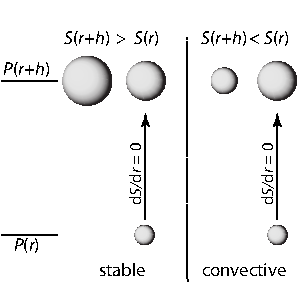
\includegraphics[width=\textwidth]{convective}
\caption[Illustration of criteria for convective instability.]{\label{f.convective-schematic}Illustration of criteria for convective instability.  On the left, raising a blob a distance $h$ adiabatically and in pressure balance with its surrounding results in a higher density $V_{b} < V$.  This is stable: the blob will sink back.  On the right, the blob is less dense and hence buoyant: it will continue to rise.}
\end{marginfigure}

Taking $h$ to be an infinitesimal displacement and expanding the left-hand side of equation~(\ref{e.archimedes}) gives us a local condition for stability:
\begin{equation}\label{e.convective-stability}
V[P(r+h),S(r)] + \tderiv{V}{S}{P}\frac{\dif S}{\dif r} - V[P(r+h),S(r)]  = \tderiv{V}{S}{P}\frac{\dif S}{\dif r} > 0 .
\end{equation}
Noting that
\begin{eqnarray*}
\tderiv{V}{T}{P} &=& \tderiv{V}{S}{P}\tderiv{S}{T}{P}\\
 &=& \frac{C_{P}}{T}\tderiv{V}{S}{P},
 \end{eqnarray*}
 we can rewrite equation~(\ref{e.convective-stability}) as
 \[
 \frac{T}{C_{P}}\tderiv{V}{T}{P}\frac{\dif S}{\dif r} > 0.
 \]
Now, $(\partial V/\partial T)_{P}$ is positive (gas expands on being heated), so our condition for stability is simply
 \begin{equation}\label{e.entropy-condition}
\frac{\dif S}{\dif r} > 0.
\end{equation}
In a convectively stable star, the entropy must increase with radius. if $\dif S/\dif r < 0$, then convection occurs and carries high-entropy material outward, where it will eventually mix with the ambient medium.  As a result, convection drives the entropy gradient toward the marginally stable configuration $\dif S/\dif r = 0$.  If a star is fully convective and mixes efficiently, then the interior of the star lies along an adiabat. 

\newthought{We can derive a condition for convective stability} in terms of the local gradients of temperature and pressure. Writing $S = S[P(r),T(r)]$ we expand equation~(\ref{e.entropy-condition}) to obtain
\begin{equation}\label{e.schwarzschild-1}
\frac{\dif S}{\dif r} = \tderiv{S}{P}{T} \frac{\dif P}{\dif r} + \tderiv{S}{T}{P}\frac{\dif T}{\dif r} .
\end{equation}
Now, $P$ is a monotonically decreasing function of $r$, which means we can change variables:
\begin{equation}\label{e.TPstar}
\frac{\dif T}{\dif r} = \TPstar \frac{\dif P}{\dif r} .
\end{equation}
Here $\dif T/\dif P|_{\star}$ is the slope of the $T(P)$ relation \emph{for the stellar interior}.  In particular, this is \emph{not} a thermodynamic equality. Substituting equation~(\ref{e.TPstar}) into equation~(\ref{e.schwarzschild-1}), using hydrostatic equilibrium to eliminate $\dif P/\dif r$, and recognizing that $(\partial S/\partial T)_{P} = C_{P}/T$, we obtain
\begin{equation}\label{e.schwarzschild-2}
\frac{\dif S}{\dif r} =  -\rho g\left[\tderiv{S}{P}{T} + \frac{C_{P}}{T} \TPstar \right].
\end{equation}
Finally, we can use the identity
\begin{equation}
\tderiv{S}{P}{T}\tderiv{T}{S}{P}\tderiv{P}{T}{S} = -1
\end{equation}
to simplify equation~(\ref{e.schwarzschild-2}),
\begin{equation}
\frac{\dif S}{\dif r} = -\frac{\rho g}{P}C_{P}\left[\frac{P}{T}\TPstar - \frac{P}{T}\tderiv{T}{P}{S}\right].
 \label{e.schwarzschild}
\end{equation}
Hence, if the term in $\left[\cdot\right]$ is positive, then the fluid is convectively unstable.

Let's use our expression for the flux, Equation~(\ref{e.gradient-temperature}), to put $\left.\dif T/\dif P\right|_\star$ in terms of $\kappa$ and $L(r)$:
\begin{eqnarray}
    \frac{P}{T}\TPstar &=& \frac{P}{T}\DD{T}{r}\DD{r}{P} = \frac{P}{\rho g(r)}\frac{1}{\color{red}T}\frac{{\color{red}3}\rho\kappa}{4c {\color{red}a T^3}}\frac{L(r)}{4\pi r^2} \nonumber\\
    &=& \frac{P}{\color{red}\Prad}\frac{\kappa}{16\pi Gc} \frac{L(r)}{m(r)}.
\end{eqnarray}
The fluid is unstable to convection if
\begin{equation}
    \frac{P}{\Prad}\frac{\kappa}{16\pi Gc}\frac{L(r)}{m(r)} > \tderiv{\ln T}{\ln P}{S}  = \frac{\gamma -1}{\gamma}.
\end{equation}
We have used Equation~(\ref{e.nabla-adiabat}) for the last term here.
This occurs for large $\kappa$ (outer layers of cool stars) or for a high $L(r)/m(r)$ (centers of luminous hot stars).  On the main-sequence, stars with $M \lesssim \Msun$ have convective outer layers; stars with $M \lesssim \val{0.3}{\Msun}$ are fully convective. Stars with $M\gtrsim\Msun$ have convective cores.